\documentclass{aastex61}


%% arguement options are:
%%
%%  twocolumn   : two text columns, 10 point font, single spaced article.
%%                This is the most compact and represent the final published
%%                derived PDF copy of the accepted manuscript from the publisher
%%  manuscript  : one text column, 12 point font, double spaced article.
%%  preprint    : one text column, 12 point font, single spaced article.  
%%  preprint2   : two text columns, 12 point font, single spaced article.
%%  modern      : a stylish, single text column, 12 point font, article with
%% 		  wider left and right margins. This uses the Daniel
%% 		  Foreman-Mackey and David Hogg design.
%%
%% Note that you can submit to the AAS Journals in any of these 6 styles.
%%
%% There are other optional arguments one can envoke to allow other stylistic
%% actions. The available options are:
%%
%%  astrosymb    : Loads Astrosymb font and define \astrocommands. 
%%  tighten      : Makes baselineskip slightly smaller, only works with 
%%                 the twocolumn substyle.
%%  times        : uses times font instead of the default
%%  linenumbers  : turn on lineno package.
%%  trackchanges : required to see the revision mark up and print its output
%%  longauthor   : Do not use the more compressed footnote style (default) for 
%%                 the author/collaboration/affiliations. Instead print all
%%                 affiliation information after each name. Creates a much
%%                 long author list but may be desirable for short author papers
%%
%% these can be used in any combination, e.g.
%%
%% \documentclass[twocolumn,linenumbers,trackchanges]{aastex61}

\usepackage{graphicx}
\usepackage{amssymb}
\usepackage{color}
\usepackage{breakurl}

\usepackage{amsthm, amsmath}
\def\UrlFont{\sf}
\let\captionbox\relax
\usepackage[caption=false]{subfig}

\usepackage{tikz}
\usetikzlibrary{decorations.markings}


%% Definitions for the journal names
%\newcommand{\adv}{    {\it Adv. Space Res.}} 
%\newcommand{\annG}{   {\it Ann. Geophys.}} 
%\newcommand{\aap}{    {\it Astron. Astrophys.}}
%\newcommand{\aaps}{   {\it Astron. Astrophys. Suppl.}}
%\newcommand{\aapr}{   {\it Astron. Astrophys. Rev.}}
%\newcommand{\ag}{     {\it Ann. Geophys.}}
%\newcommand{\aj}{     {\it Astron. J.}} 
%\newcommand{\apj}{    {\it Astrophys. J.}}
%\newcommand{\apjl}{   {\it Astrophys. J. Lett.}}
%\newcommand{\apss}{   {\it Astrophys. Space Sci.}} 
%\newcommand{\cjaa}{   {\it Chin. J. Astron. Astrophys.}} 
%\newcommand{\gafd}{   {\it Geophys. Astrophys. Fluid Dyn.}}
%\newcommand{\grl}{    {\it Geophys. Res. Lett.}}
%\newcommand{\ijga}{   {\it Int. J. Geomagn. Aeron.}}
%\newcommand{\jastp}{  {\it J. Atmos. Solar-Terr. Phys.}} 
%\newcommand{\jgr}{    {\it J. Geophys. Res.}}
%\newcommand{\lrsp}{Living Rev. Solar Phys.}
%\newcommand{\mnras}{  {\it Mon. Not. Roy. Astron. Soc.}}
%\newcommand{\nat}{    {\it Nature}}
%\newcommand{\pasp}{   {\it Pub. Astron. Soc. Pac.}}
%\newcommand{\pasj}{   {\it Pub. Astron. Soc. Japan}}
%\newcommand{\pre}{    {\it Phys. Rev. E}}
%\newcommand{\solphys}{{\it Solar Phys.}}
%\newcommand{\sovast}{ {\it Soviet  Astron.}} 
%\newcommand{\ssr}{    {\it Space Sci. Rev.}}


%\received{July 1, 2016}
%\revised{September 27, 2016}
%\accepted{\today}
%\submitjournal{ApJ}


%%%%%%%%%%%%%%%%%%%%%%%%%%%%%%%%%%%%%%%%%%%%%%%%%%%%%%%%%%%%%%%%%%%%%%%%%%%%%%%%
%%
\shorttitle{Evolution of Asymmetric MHD Waves}
\shortauthors{Allcock and Erd\'{e}lyi}
\watermark{DRAFT}
%%
%%%%%%%%%%%%%%%%%%%%%%%%%%%%%%%%%%%%%%%%%%%%%%%%%%%%%%%%%%%%%%%%%%%%%%%%%%%%%%%%

\begin{document}
\title{Evolution of Asymmetric Slab Magnetohydrodynamic Waves}

%% LaTeX will automatically break titles if they run longer than
%% one line. However, you may use \\ to force a line break if
%% you desire. In v6.1 you can include a footnote in the title.

%% A significant change from earlier AASTEX versions is in the structure for 
%% calling author and affilations. The change was necessary to implement 
%% autoindexing of affilations which prior was a manual process that could 
%% easily be tedious in large author manuscripts.
%%
%% The \author command is the same as before except it now takes an optional
%% arguement which is the 16 digit ORCID. The syntax is:
%% \author[xxxx-xxxx-xxxx-xxxx]{Author Name}
%%
%% This will hyperlink the author name to the author's ORCID page. Note that
%% during compilation, LaTeX will do some limited checking of the format of
%% the ID to make sure it is valid.
%%
%% Use \affiliation for affiliation information. The old \affil is now aliased
%% to \affiliation. AASTeX v6.1 will automatically index these in the header.
%% When a duplicate is found its index will be the same as its previous entry.
%%
%% Note that \altaffilmark and \altaffiltext have been removed and thus 
%% can not be used to document secondary affiliations. If they are used latex
%% will issue a specific error message and quit. Please use multiple 
%% \affiliation calls for to document more than one affiliation.
%%
%% The new \altaffiliation can be used to indicate some secondary information
%% such as fellowships. This command produces a non-numeric footnote that is
%% set away from the numeric \affiliation footnotes.  NOTE that if an
%% \altaffiliation command is used it must come BEFORE the \affiliation call,
%% right after the \author command, in order to place the footnotes in
%% the proper location.
%%
%% Use \email to set provide email addresses. Each \email will appear on its
%% own line so you can put multiple email address in one \email call. A new
%% \correspondingauthor command is available in V6.1 to identify the
%% corresponding author of the manuscript. It is the author's responsibility
%% to make sure this name is also in the author list.
%%
%% While authors can be grouped inside the same \author and \affiliation
%% commands it is better to have a single author for each. This allows for
%% one to exploit all the new benefits and should make book-keeping easier.
%%
%% If done correctly the peer review system will be able to
%% automatically put the author and affiliation information from the manuscript
%% and save the corresponding author the trouble of entering it by hand.

\correspondingauthor{Robert Erd\'{e}lyi}
\email{robertus@sheffield.ac.uk}

\author[0000-0002-0771-743X]{Matthew Allcock}
\affil{Solar Physics and Space Plasma Research Centre, School of Mathematics and Statistics, University of Sheffield, Hicks Building, Hounsfield Road, Sheffield, S3 7RH, UK}

\author[0000-0003-3439-4127]{Robert Erd\'{e}lyi}
\affiliation{Solar Physics and Space Plasma Research Centre, School of Mathematics and Statistics, University of Sheffield, Hicks Building, Hounsfield Road, Sheffield, S3 7RH, UK}


\begin{abstract}

Abstract (250 word limit for ApJ)

\end{abstract}

\keywords{magnetohydrodynamics --- plasmas --- Sun: atmosphere --- Sun: oscillations --- waves}

\section{Introduction} \label{sec:intro}
Numerical results: \cite{ter_etal06}

Physicality of the principle leaky kink mode: \cite{cal03} solved the initial value problem of transverse waves in a cold magnetic flux tube. \cite{rud_etal06} repeated it showing PLK modes are on an unphysical banch of the complex plane (?). Commented on by \cite{cal06} and in return by \cite{rud_etal06b}. Settled (?) by considering numerical solution by \cite{ter_etal07} and analytically by \cite{and_etal07}. So PLK modes are not physical.

\section{initial value problem - incompressible magnetic slab}

Consider an equilibrium plasma with magnetic field $B_0(x)\mathbf{\hat{z}}$, density $\rho_0(x)$, and pressure $p_0(x)$, without gravity. In the absence of structuring in the $z$-direction and considering perturbations in the $(x,z)$-plane only, we can take Fourier components for velocity and other parameters like $\mathbf{v}(\mathbf{x},t) = \mathbf{\hat{v}}(x)e^{i(kz + ly - \omega t)}$. The velocity perturbation amplitude in the inhomogeneous direction of an ideal plasma is given by
\begin{equation}
\frac{d}{dx}\left(\frac{\epsilon(x)}{l^2 + m_0^2(x)} \frac{d\hat{v}_x}{dx}\right) - \epsilon(x)\hat{v}_x = 0,
\label{gov gen}
\end{equation}
where
\begin{equation}
\epsilon(x) = \rho_0(x)[k^2v_A^2(x)-\omega^2], \quad
m_0^2(x) = \frac{(k^2c_0^2(x) - \omega^2)(k^2v_A^2(x) - \omega^2)}{(c_0^2(x) + v_A^2(x))(k^2c_T^2(x) - \omega^2)},
\end{equation}
and
\begin{equation}
c_0(x) = \sqrt{\frac{\gamma p_0(x)}{\rho_0(x)}}, \quad
v_A(x) = \frac{B_0(x)}{\sqrt{\mu \rho_0(x)}}, \quad
c_T(x) = \frac{c_0(x)v_A(x)}{\sqrt{c_0^2(x) + v_A^2(x)}}
\end{equation} are the sound, Alfv\'{e}n, and tube speeds, respectively.

When the plasma is incompressible, so that $c_0 \to \infty$, we have $c_T^2 \to v_A^2$ and $m_0^2 \to k^2$. After restricting the analysis to propagation only parallel to the magnetic field ($l = 0$), Equation~\eqref{gov gen} reduces to
\begin{equation}
\frac{d}{dx}\left(\epsilon(x) \frac{d\hat{v}_x}{dx}\right) - k^2\epsilon(x)\hat{v}_x = 0,
\label{gov}
\end{equation}
which is commonly used for solving eigenmode problems in MHD wave physics. In the present work, the temporal evolution of linear asymmetric MHD waves is considered so we must dial back our assumptions about how the wave behaviour through time.

Above we used a Fourier decomposition in time, which is valid when the solutions are homogeneous in time, such as normal mode solutions (rewrite this). To investigate the temporal evolution of solutions, we take only Fourier components in the $z$-direction, that is $\mathbf{v}(\mathbf{x},t) = \mathbf{\hat{v}}(x,t)e^{ikz}$, and we take the Laplace transform with respect to time, such that
\begin{equation}
\mathbf{\tilde{v}}(x) = \int_0^\infty \mathbf{\widehat{v}}(x,t)e^{i\omega t} dt.
\end{equation}
This gives us the initial-value form of Equation~\eqref{gov} to be
\begin{equation}
\frac{d}{dx}\left(\epsilon(x) \frac{d\tilde{v}_x}{dx}\right) - k^2\epsilon(x)\tilde{v}_x = f(x),
\label{ivp gov}
\end{equation}
where
\begin{equation}
f(x) = ik\left\{\rho_0\left[\frac{\partial\hat{\Omega}}{\partial t}(x,0) - i\omega\hat{\Omega}(x,0)\right] - \left[\frac{\partial\hat{v}_z}{\partial t}(x,0) - i\omega \hat{v}_z(x,0)\right]\frac{d\rho_0}{dx}\right\},
\label{f}
\end{equation}
where the vorticity, $\Omega(x,t)\mathbf{\hat{y}} = \hat{\Omega}(x,t)e^{ikz}\mathbf{\hat{y}} = \nabla \times \mathbf{v}(\mathbf{x},t)$, is given by
\begin{equation}
\hat{\Omega}(\mathbf{x},t) = -\frac{i}{k}\left(\frac{\partial^2\hat{v}_x}{\partial x^2} - k^2 \hat{v}_x\right).
\end{equation}
(this differs from \cite{rae_etal81} by a factor of $-1$ due to taking Fourier forms like $e^{ikz}$ rather than $e^{-ikz}$)

Consider equilibrium magnetic field and density profiles given by
\begin{equation}
B(x)=
\begin{cases}
B_1, & \text{if  }x<-x_0, \\
B_0, & \text{if }|x|\leq{x_0}, \\
B_2, & \text{if  }x>x_0,
\end{cases}
\quad \text{and} \quad
\rho(x)=
\begin{cases}
\rho_1, & \text{if  }x<-x_0, \\
\rho_0, & \text{if }|x|\leq{x_0}, \\
\rho_2, & \text{if  }x>x_0,
\end{cases}
\end{equation}
where $B_i$ and $\rho_i$ are uniform for $i = 0,1,2$. This establishes the plasma as magnetic slab embedded in an asymmetric magnetic background.

In this equilibrium, transverse velocity perturbations are related to initial perturbations in the following way:
\begin{equation}
\frac{d^2\tilde{v}_x}{dx^2} - k^2\tilde{v}_x = 
\begin{cases}
f(x)/\epsilon_1, & \text{if  } x<-x_0,\\
f(x)/\epsilon_0, & \text{if  } |x|<x_0,\\
f(x)/\epsilon_2, & \text{if  } x>x_0.
\end{cases}
\label{ivp gov slab}
\end{equation}


\subsection{Attempt 1}
Sturm-Liouville Theory tells us that with the aid of a Green's function, $G(x;s)$, Equation~\eqref{ivp gov slab} can be solved to give
\begin{equation}
\tilde{v}_x(x) =
\begin{cases}
\tilde{A}(\cosh{kx} + \sinh{kx}) - \frac{1}{\epsilon_1} \int_{-\infty}^{-x_0} G(x;s)f(s)ds, & \text{if  } x<-x_0,\\
\tilde{B}\cosh{kx} + \tilde{C}\sinh{kx} - \frac{1}{\epsilon_0} \int_{-x_0}^{x_0} G(x;s)f(s)ds, & \text{if  } |x|<x_0,\\
\tilde{D}(\cosh{kx} - \sinh{kx}) - \frac{1}{\epsilon_2} \int_{x_0}^{\infty} G(x;s)f(s)ds, & \text{if  } x>x_0,
\end{cases}
\label{ivp slab sol}
\end{equation}
where
\begin{equation}
G(x;s) = \frac{1}{2k}[e^{ks}e^{-kx}H(x-s) + e^{-ks}e^{kx}H(s-x)]
\end{equation}
and $H$ is the Heaviside step function. Ensuring continuity of both transverse velocity and total pressure across the boundaries at $x=\pm x_0$ gives us the following system of linear algebraic equations for the constants $A$, $B$, $C$, and $D$:
\begin{equation}
\left(
\begin{matrix}
c_0-s_0              &-c_0           &s_0              &0                   \\
0                    &c_0            &s_0              &s_0-c_0           \\
\epsilon_1(c_0-s_0)  &\epsilon_0s_0  &-\epsilon_0c_0   &0                   \\
0                    &\epsilon_0s_0  &\epsilon_0c_0    &-\epsilon_2(s_0-c_0)
\end{matrix}
\right)
\left(
\begin{matrix}
\tilde{A} \\
\tilde{B} \\
\tilde{C} \\
\tilde{D}
\end{matrix}
\right)
=
\frac{1}{2k}
\left(
\begin{matrix}
e^{kx_0}/\epsilon_1  & -e^{-kx_0}/\epsilon_0  & 0                      & 0                   \\
0                    & 0                      & e^{-kx_0}/\epsilon_0   & -e^{kx_0}/\epsilon_2 \\
-e^{kx_0} & -e^{-kx_0}  & 0                      & 0                   \\
0                    & 0                      & -e^{-kx_0}  & -e^{kx_0}
\end{matrix}
\right)
\left(
\begin{matrix}
I_1    \\
I_0^- \\
I_0^+ \\
I_2
\end{matrix}
\right),
\label{coefmatrix}
\end{equation}
where $c_0 = \cosh{kx_0}$, $s_0 = \sinh{kx_0}$, and the functionals $I_1$, $I_0^-$, $I_0^+$, and $I_2$ are given by
\begin{equation}
I_1 = \int_{-\infty}^{-x_0} e^{ks}f(s) ds, \quad I_0^- = \int_{-x_0}^{x_0} e^{-ks}f(s) ds, \quad I_0^+ = \int_{-x_0}^{x_0} e^{ks}f(s) ds, \quad I_2  = \int_{x_0}^{\infty} e^{-ks}f(s) ds.
\end{equation}
Solving this system of equations gives
\newcommand{\e}{\epsilon}
\begin{equation}
\tilde{A} = \frac{e^{2kx_0}T_1}{2k\e_1D_R}, 
\quad 
\tilde{B} = \frac{e^{2kx_0}T_0^-}{2k\e_0D_R}, 
\quad 
\tilde{C} = \frac{e^{2kx_0}T_0^+}{2k\e_0D_R}, 
\quad 
\tilde{D} = \frac{e^{2kx_0}T_2}{2k\e_2D_R},
\label{consts}
\end{equation}
where
\begin{align}
T_1(\omega) &= I_1[e^{4kx_0}(\e_0 - \e_1)(\e_0 + \e_2) - (\e_0 + \e_1)(\e_0 - \e_2)]- 4I_2e^{2kx_0}\e_0\e_1 - 2\e_1\left[I_0^-e^{2kx_0}(\e_0 + \e_2) + I_0^+(\e_0 - \e_2)\right], \\
T_0^-(\omega) &= [(I_0^+ - I_0^-)(\e_2 - \e_1)\e_0 - (I_0^+ + I_0^-)(\e_0^2 - \e_1\e_2)]e^{2kx_0} - (I_0^+ + I_0^-)(\e_0 - \e_1)(\e_0 - \e_2) \notag \\
& \quad - 2\e_0e^{2kx_0}\left[((I_1 + I_2)\e_0 + I_1\e_2 + I_2\e_1)e^{2kx_0} + (I_1 + I_2)\e_0 - I_1\e_2 - I_2\e_1\right], \\
T_0^+(\omega) &= [(I_0^+ + I_0^-)(\e_2 - \e_1)\e_0 - (I_0^+ - I_0^-)(\e_0^2 - \e_1\e_2)]e^{2kx_0} - (I_0^+ - I_0^-)(\e_0 - \e_1)(\e_0 - \e_2) \notag \\
& \quad - 2\e_0e^{2kx_0}\left[((I_2 - I_1)\e_0 - I_1\e_2 + I_2\e_1)e^{2kx_0} + (I_1 - I_2)\e_0 - I_1\e_2 + I_2\e_1\right], \\
T_2(\omega) &= I_2[e^{4kx_0}(\e_0 + \e_1)(\e_0 - \e_2) - (\e_0 - \e_1)(\e_0 + \e_2)] - 4I_1e^{2kx_0}\e_0\e_2 -  2\e_2\left[I_0^+e^{2kx_0}(\e_0 + \e_1) + I_0^-(\e_0 - \e_1)\right], \\
D_R(\omega) &= (\e_0 + \e_1)(\e_0 + \e_2)e^{4kx_0} - (\e_0 - \e_1)(\e_0 - \e_2).
\label{DR incomp}
\end{align}

The solutions of equation $D_R(\omega) = 0$ are precisely the solutions of the dispersion relation for an incompressible asymmetric magnetic slab. To confirm this, we follow notion from \cite{zsa_etal18} (with an added superscript~$z$) by observing that for an incompressible plasma, the sound speed, $c_s \to \infty$. Therefore,
\begin{equation}
m_j^2 = \frac{(k^2c_j^2 - \omega^2)(k^2v_{Aj}^2 - \omega^2)}{(c_j^2 + v_{Aj}^2)(k^2c_Tj^2 - \omega^2)} \to k^2,
\end{equation}
\begin{equation}
\Lambda_j^z = \frac{i\rho_j}{\omega m_j}(k^2v_{Aj}^2 - \omega^2) \to \frac{i \rho_j}{\omega k}(k^2v_{Aj}^2 - \omega^2), \quad \text{for } j = 0,1,2.
\end{equation}
Therefore, after multiplying Equation~\eqref{DR incomp} by $\omega k / i(e^{4kx_0} + 1)$, we recover the dispersion relation in \cite{zsa_etal18} for an incompressible plasma, namely
\begin{equation}
2(\Lambda_0^2 + \Lambda_1\Lambda_2) + \Lambda_0(\Lambda_1 + \Lambda_2)[\tanh{kx_0} + \coth{kx_0}] = 0.
\end{equation}

The solution given by Equation~\eqref{ivp slab sol}, with constants (with respect to $x$) $\tilde{A}$, $\tilde{B}$, $\tilde{C}$, and $\tilde{D}$, given by Equation~\eqref{consts} corroborates with those describing the initial value problem of surface waves on an interface between two incompressible plasmas. When the slab width, $2x_0$, approaches zero, it is expected that the solutions here approach those describing the interface. As $x_ 0 \to 0$, the dispersion function behaves like
\begin{equation}
D_R \to (\epsilon_0 + \epsilon_1)(\epsilon_0 + \epsilon_2) - (\epsilon_0 - \epsilon_1)(\epsilon_0 - \epsilon_2) = 2\epsilon_0(\epsilon_1 + \epsilon_2).
\end{equation}
Therefore, in this limit, $\tilde{A}$ and $\tilde{D}$ behave like
\begin{align}
\tilde{A} &\to \frac{1}{4k\epsilon_0\epsilon_1(\epsilon_1 + \epsilon_2)} \left\{ 2I_1\epsilon_0(\epsilon_2 - \epsilon_1) - 4I_2\epsilon_0\epsilon_1 \right\} = \frac{1}{k(\epsilon_1 + \epsilon_2)} \left\{ -I_2 + \frac{1}{2\epsilon_1}(\epsilon_2 - \epsilon_1)I_1 \right\}, \\
\tilde{D} &\to \frac{1}{4k\epsilon_0\epsilon_2(\epsilon_1 + \epsilon_2)} \left\{ 2I_2\epsilon_0(\epsilon_1 - \epsilon_2) - 4I_1\epsilon_0\epsilon_2 \right\} = \frac{1}{k(\epsilon_1 + \epsilon_2)} \left\{ -I_1 + \frac{1}{2\epsilon_2}(\epsilon_1 - \epsilon_2)I_2 \right\}, \\
\end{align}
which are equal to (the corrected versions of) $A_-$ and $A_+$, respectively, from \cite{rae_etal81}.



\subsubsection{Solution in time}

To recover the transverse velocity, $v_x(x, t)$, we employ the inverse Laplace transform, such that
\begin{equation}
v_x(x,t) = \frac{1}{2\pi} \lim_{L \to \infty} \int_{i\gamma - L}^{i\gamma + L} \tilde{v}_x(x,\omega) e^{-i\omega t} d\omega,
\end{equation}
where $\gamma$ is a real number such that all the singularities of the integrand is below the contour of integration. The integral is evaluated along an infinite horizontal line in the upper half of the complex plane. Since the problem is now reduced to solving a complex integral, it is dependent on the singularities (with respect to $\omega$) of $\tilde{v}_x$, whose residues determine the value of the contour integral.

Focusing firstly on the region $x<-x_0$, the solution is
\begin{align}
v_x &= \frac{1}{2\pi} \lim_{L \to \infty} \int_{i\gamma - L}^{i\gamma + L} \left[ \tilde{A}e^{k(x+x_0)} + \frac{1}{\e_1} \int_{-\infty}^{-x_0} G(x;s)f(s)ds \right]e^{-i\omega t} d\omega, \\
&= \frac{e^{k(x+x_0)}}{2\pi} \left( \lim_{L \to \infty} \int_{i\gamma - L}^{i\gamma + L} \tilde{A} e^{-i\omega t} ds \right) + \left(\int_{-\infty}^{-x_0} G(x;s)f(s)ds \right) \left( \lim_{L \to \infty} \int_{i\gamma - L}^{i\gamma + L} \frac{e^{-i\omega t}}{\e_1} d\omega \right),
\label{sol incomp}
\end{align}

The first integral in the above solution is calculated as follows:
The functions $\epsilon_{0,1,2}$ are polynomial in $\omega$, and are therefore entire. The integrals $I_{1,2}$ and $I_0^\pm$ are not functions of $\omega$ so also contribute no singularities in $\omega$. Therefore, $T_{1,2}$, and $T_0^\pm$ are entire functions.

The final integral in Equation~\eqref{sol incomp} is calculated as follows:


the singularities of $\tilde{v}_x$ are precisely the singularities of $A$ and $1/\e_1$

Considering the functional form of $\tilde{v}_x(x, \omega)$, we see that, in each region, it is made up of a term involving 










































\subsubsection{Specific initial conditions}
The above approach using arbitrary initial conditions is forced to cease here due to mathematical intractability of the general inverse Laplace transform calculation (however, general asymptotic results are, just barely, tractable). Instead, we progress with specific initial conditions. 

Choosing specific initial conditions requires a delicate balance between mathematical tractability and physical applicability. 
















\subsection{Attempt 2}

The idea behind this second attempt is to choose the Green's function in such a way as to make the constant coefficients of the particular solution part are directly related to the boundary values of the transverse velocity.

We are trying to solve the equation
\begin{equation}
\frac{d^2\tilde{v}_x}{dx^2} - k^2\tilde{v}_x = 
\begin{cases}
f(x)/\epsilon_1, & \text{if  } x<-x_0,\\
f(x)/\epsilon_0, & \text{if  } |x|<x_0,\\
f(x)/\epsilon_2, & \text{if  } x>x_0,
\end{cases}
\label{ivp gov slab 2}
\end{equation}
under the boundary conditions $\tilde{v}_x(-x_0) = \tilde{A}_1$ and $\tilde{v}_x(x_0) = \tilde{A}_2$.

The Green's function, $G(x;s)$, corresponding to Equation~\eqref{ivp gov slab 2} must satisfy 
\begin{equation}
\frac{\partial^2G}{\partial x^2} - k^2 G = \delta(x-s), \quad G(-x_0;s) = G(x_0;s) = 0,
\end{equation}
where $\delta$ denotes the Dirac Delta function. It is instructive to piecewise define the Green's function as
\begin{equation}
G(x;s) = 
\begin{cases}
G_1(x;s), & \text{if } x < -x_0, \\
G_0(x;s), & \text{if } |x| < x_0, \\
G_2(x;s), & \text{if } x_0 < x.
\end{cases}
\end{equation}
The general solution, for $|x| < x_0$, of the equation for $G_0$ is
\begin{equation}
G_0(x;s) = c_1\sinh(k(x - x_0)) + c_2\sinh(k(x + x_0)),
\end{equation}
where $c_1 = 0$ for $x < s$ and $c_2 = 0$ for $x > s$. Ensuring $G_0$ and $\partial G_0 / \partial x$ have jumps of 0 and 1 at $x = s$, respectively, determines $c_1$ and $c_2$, so that $G_0(x;s)$ is
\begin{equation}
G_0(x;s) = \frac{1}{k\sinh(2k x_0)}
\begin{cases}
\sinh(k(s - x_0))\sinh(k(x + x_0)), & \text{if } -x_0<x<s, \\
\sinh(k(x - x_0))\sinh(k(s + x_0)), & \text{if } s<x<x_0.
\end{cases}
\end{equation}

Because the boundary conditions are inhomogeneous, we must add to the standard Green's function solution a term that is a solution to the homogeneous equation and the inhomogeneous boundary conditions. In this manner, we find that the solution within the slab is
\begin{equation}
\tilde{v}_x(x) = \frac{1}{\sinh{2kx_0}} \left[ \tilde{A}_1\sinh(k(x_0 - x)) + \tilde{A}_2\sinh(k(x_0 + x)) \right] + \frac{1}{\epsilon_0}\int_{-x_0}^{x_0} G_0(x;s) f(s) ds.
\end{equation}

Similarly, we find that the Green's function for the plasma outside the slab is 
\begin{equation}
G_1(x;s) = \frac{1}{k}
\begin{cases}
e^{k(x + x_0)}\sinh(k(s + x_0)), & \text{if } x < s, \\
e^{k(s + x_0)}\sinh(k(x + x_0)), & \text{if } s < x < -x_0,
\end{cases}
\end{equation}
for $x < -x_0$, and
\begin{equation}
G_2(x;s) = -\frac{1}{k}
\begin{cases}
e^{-k(s - x_0)}\sinh(k(x - x_0)), & \text{if } x_0 < x < s, \\
e^{-k(x - x_0)}\sinh(k(s - x_0)), & \text{if } s < x,
\end{cases}
\end{equation}
for $x > x_0$. Therefore the solution is
\begin{equation}
\tilde{v}_x(x) = \tilde{A}_1e^{k(x_0 + x)} + \frac{1}{\epsilon_1}\int_{-\infty}^{-x_0} G_1(x;s) f(s) ds,
\end{equation}
for $x < -x_0$, and
\begin{equation}
\tilde{v}_x(x) = \tilde{A}_2e^{k(x_0 - x)} + \frac{1}{\epsilon_2}\int_{x_0}^{\infty} G_2(x;s) f(s) ds,
\end{equation}
for $x > x_0$.


\subsubsection{Matching solutions}
To establish physically relevant solutions, we require that the transverse velocity and the total pressure are continuous over each interface. Given the above solutions, the transverse velocity is automatically continuous over the boundaries. The perturbation in the total pressure, $P_T$, for a compressible plasma is given (for example, in \cite{all_etal17}) by
\begin{equation}
\tilde{P}_T(x) = \frac{\Lambda}{m}\frac{d\tilde{v}_x}{d x},
\end{equation}
where
\begin{equation}
\Lambda = \frac{i\rho(\omega^2 - k^2v_A^2)}{m\omega},
\quad
m^2 = \frac{(k^2v_A^2 - \omega^2)(k^2c_0^2 - \omega^2)}{(c_0^2 + v_A^2)(k^2c_T^2 - \omega^2)},
\quad \text{and} \quad
c_T^2 = \frac{c_0^2 v_A^2}{c_0^2 + v_A^2}.
\end{equation}
When the plasma is incompressible, $m^2 \to k^2$, therefore continuity in total pressure is equivalent to continuity in $\epsilon(x)\tilde{v}_x'(x)$ for an incompressible plasma.

Applying this boundary condition gives
\begin{equation}
\tilde{A}_1(\omega) = \frac{T_1(\omega)}{k D(\omega)}, \quad \tilde{A}_2(\omega) = \frac{T_2(\omega)}{k D(\omega)},
\end{equation}
where
\begin{align}
T_1(\omega) & = (I_0^- - I_1)[\epsilon_0\cosh(2kx_0) + \epsilon_2\sinh(2kx_0)] - \epsilon_0(I_0^+ + I_2), \\
T_2(\omega) & = \epsilon_0(I_0^- - I_1) - (I_0^+ + I_2)[\epsilon_0\cosh(2kx_0) + \epsilon_1\sinh(2kx_0)], \\
D(\omega) & = \epsilon_0(\epsilon_1 + \epsilon_2)\cosh(2kx_0) + (\epsilon_0^2 + \epsilon_1\epsilon_2)\sinh(2kx_0),
\label{D incomp}
\end{align}
and
\begin{equation}
I_0^\pm = \int_{-x_0}^{x_0} \frac{\sinh(k(s \pm x_0))}{\sinh(2kx_0)} f(s) ds,
\quad
I_1 = \int_{-\infty}^{-x_0} e^{k(s + x_0)} f(s) ds,
\quad
I_2 = \int_{x_0}^\infty e^{k(x_0 - s)} f(s) ds.
\end{equation}


























\subsubsection{Solution in time}

To recover the transverse velocity, $v_x(x, t)$, we employ the inverse Laplace transform (non-standard, discussed in Appendix~\ref{app: laplace trans}), such that
\begin{equation}
v_x(x,t) = \frac{1}{2\pi} \lim_{L \to \infty} \int_{i\gamma - L}^{i\gamma + L} \tilde{v}_x(x,\omega) e^{-i\omega t} d\omega,
\end{equation}
where $\gamma$ is a real number such that all the singularities of the integrand is below the contour of integration. The integral is evaluated along an infinite horizontal line in the upper half of the complex plane. Since the problem is now reduced to solving a complex integral, it is dependent on the singularities (with respect to $\omega$) of $\tilde{v}_x$, whose residues determine the value of the contour integral.

Focusing firstly on the region $x<-x_0$, the solution is
\begin{align}
v_x &= \frac{1}{2\pi} \lim_{L \to \infty} \int_{i\gamma - L}^{i\gamma + L} \left[ \tilde{A}_1 e^{k(x+x_0)} + \frac{1}{\e_1} \int_{-\infty}^{-x_0} G_1(x;s)f(s)ds \right]e^{-i\omega t} d\omega, \\
&= \frac{e^{k(x+x_0)}}{2\pi} \left( \lim_{L \to \infty} \int_{i\gamma - L}^{i\gamma + L} \tilde{A}_1 e^{-i\omega t} ds \right) + \left(\int_{-\infty}^{-x_0} G_1(x;s)f(s)ds \right) \left( \lim_{L \to \infty} \int_{i\gamma - L}^{i\gamma + L} \frac{e^{-i\omega t}}{\e_1} d\omega \right),
\label{sol incomp}
\end{align}

The first integral in the above solution is calculated as follows. The functions $\epsilon_{0,1,2}$ are polynomial in $\omega$, and are therefore entire. The integrals $I_{1,2}$ and $I_0^\pm$ are not functions of $\omega$ so also contribute no singularities in $\omega$. Therefore, $T_1$ and $T_2$ are entire functions.

The zeros of $D(\omega)$ are determined by firstly noting that $D=0$ is the dispersion relation of the corresponding eigenvalue problem solved by \cite{zsa_etal18}. They show that the dispersion relation governing transverse wave propagation parallel to the magnetic field in an asymmetric slab of compressible plasma is given by
\begin{equation}
2(\Lambda_0^2 + \Lambda_1 \Lambda_2) + \Lambda_0(\Lambda_1 + \Lambda_2)[\tanh(m_0x_0) + \coth(m_0x_0)] = 0,
\label{DR}
\end{equation}
where
\begin{equation}
\Lambda_j = -\frac{i\rho_j(k^2v_{Aj}^2 - \omega^2)}{\omega m_j},
\quad
m_j^2 = \frac{(k^2c_j^2 - \omega^2)(k^2v_{Aj}^2 - \omega^2)}{(c_j^2 + v_{Aj}^2)(k^2c_{Tj}^2 - \omega^2)},
\quad
\text{and}
\quad
c_{Tj}^2 = \frac{c_j^2v_{Aj}^2}{c_j^2 + v_{Aj}^2},
\end{equation}
for $j = 0, 1, 2$. When compressibility is neglected, such that the sound speeds, $c_j$, approach infinity, we have $c_{Tj}^2 \to v_{Aj}^2$, $m_j^2 \to k^2$, and therefore $\Lambda_j = -i\rho_j(k^2v_{Aj}^2 - \omega^2)/\omega k = -i\epsilon_j / \omega k$, for $j=0,1,2$. Therefore, Equation~\eqref{DR} can be reduced to the dispersion relation for an incompressible magnetic slab, which is
\begin{equation}
2(\epsilon_0^2 + \epsilon_1 \epsilon_2) + \epsilon_0(\epsilon_1 + \epsilon_2)[\tanh(m_0x_0) + \coth(m_0x_0)] = 0,
\end{equation}
which can easily to shown to be equivalent to $D(\omega) = 0$, where $D(\omega)$ is given by Equation~\eqref{D incomp}. It follows that the zeros of $D(\omega)$ are precisely the eigenvalues of the asymmetric incompressible magnetic slab.

The zeros of $D(\omega) = 0$ are found by writing this equation as
\begin{equation}
\epsilon_0(\epsilon_1 + \epsilon_2) + (\epsilon_0^2 + \epsilon_1\epsilon_2)\tanh(2kx_0) = 0
\end{equation}
and substituting expressions for $\epsilon(x)$, which gives
\begin{equation}
\rho_0(k^2v_{A0}^2 - \omega^2)[\rho_1(k^2v_{A1}^2 - \omega^2) + \rho_2(k^2v_{A2}^2 - \omega^2)] + [\rho_0^2(k^2v_{A0}^2 - \omega^2)^2 + \rho_1\rho_2(k^2v_{A1}^2 - \omega^2)(k^2v_{A2}^2 - \omega^2)]\tanh(2kx_0) = 0.
\end{equation}
The above equation can be rewritten as a quadratic in $(\omega/k)^2$, namely
\begin{align}
& \left(\frac{\omega}{k}\right)^4 [(\rho_0^2 + \rho_1\rho_2)\tanh(2kx_0) + \rho_0(\rho_1 + \rho_2)]  \\
- & \left(\frac{\omega}{k}\right)^2 [(2\rho_0^2v_{A0}^2 + \rho_1\rho_2(v_{A1}^2 + v_{A2}^2))\tanh(2kx_0) + \rho_0v_{A0}^2(\rho_1 +\rho_2) + \rho_0(\rho_1v_{A1}^2 + \rho_2v_{A2}^2)] \\
+ & [(\rho_0^2v_{A0}^4 + \rho_1\rho_2v_{A1}^2v_{A2}^2)\tanh(2kx_0) + \rho_0v_{A0}^2(\rho_1v_{A1}^2 + \rho_2v_{A2}^2)] = 0,
\end{align}
which has solutions
\begin{equation}
\left(\frac{\omega_0}{k}\right)^2 = \frac{-b \pm \sqrt{b^2 - 4ac}}{2a}, \label{solution omega0}
\end{equation}
where
\begin{align}
a &= (\rho_0^2 + \rho_1\rho_2)\tanh(2kx_0) + \rho_0(\rho_1 + \rho_2), \label{solution a} \\
b &= (2\rho_0^2v_{A0}^2 + \rho_1\rho_2(v_{A1}^2 + v_{A2}^2))\tanh(2kx_0) + \rho_0v_{A0}^2(\rho_1 +\rho_2) + \rho_0(\rho_1v_{A1}^2 + \rho_2v_{A2}^2), \label{solution b} \\
c &= (\rho_0^2v_{A0}^4 + \rho_1\rho_2v_{A1}^2v_{A2}^2)\tanh(2kx_0) + \rho_0v_{A0}^2(\rho_1v_{A1}^2 + \rho_2v_{A2}^2). \label{solution c}
\end{align}

The solutions, $\omega_0$ corroborate with the corresponding incompressible eigenfrequencies for an interface and a symmetric slab, as shown in Appendices~\ref{app: interface} and~\ref{app: symmetric}, respectively.

Given that the function $T_1(\omega)$ is entire, we can construct a closed Bromwich contour, $C = C_0 + C_1$, where $C_0$ is a straight line from $(-L, \gamma)$ to $(L, \gamma)$, and $C_1$ connects $(-L, \gamma)$ and $(L, \gamma)$ via a semi-circle to ensure that $C$ encloses the zeros of $D$ at $\pm\omega_0$, as shown by Figure~\ref{fig: brom cont incomp} (WHY IS THIS HAPPENING?!).

\begin{figure}
	\centering
	\scalebox{0.9}{
		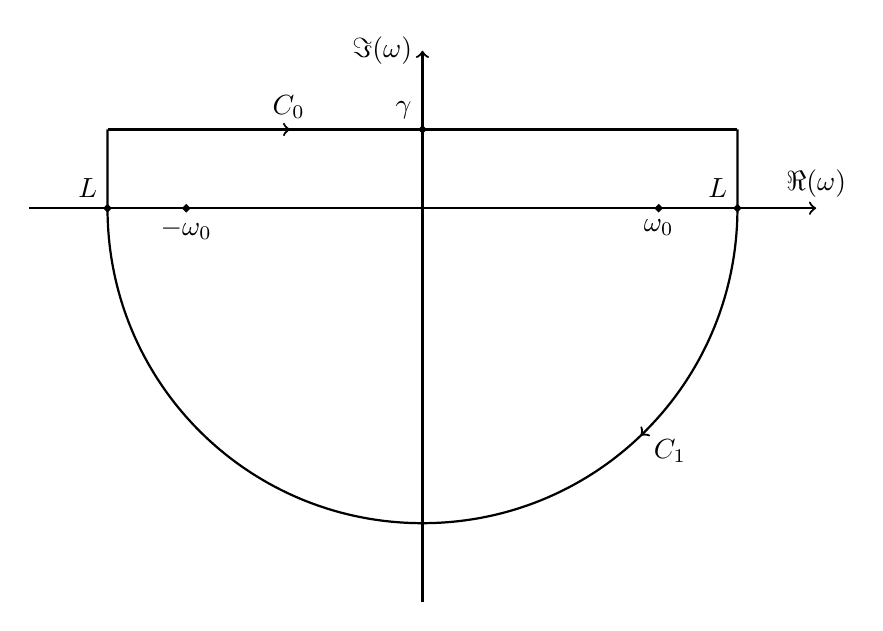
\begin{tikzpicture}[very thick,decoration={
			markings,
			mark=at position 0.29 with {\arrow{>}}}
		]
		\draw [->, thick] (-5,0) -- (5,0) node[above]{$\Re(\omega)$};
		\draw [->, thick] (0,-5) -- (0,2) node[left]{$\Im(\omega)$};
		
		\draw [postaction={decorate}, thick] (-4,1) -- (4,1);
		\draw [postaction={decorate}, thick] (4,1) to (4,0) node[above left]{$L$} to [out=-90,in=0] (0,-4) to [out=180,in=-90] (-4,0) node[above left]{$L$} to (-4,1);
		\node [above left] at (0,1) {$\gamma$};
		
		\draw[fill] (-4,0) circle [radius=0.025];
		\draw[fill] (4,0) circle [radius=0.025];
		\draw[fill] (0,1) circle [radius=0.025];
		
		\draw[fill] (3,0) circle [radius=0.025];
		\node [below] at (3,0) {$\omega_0$};
		
		\draw[fill] (-3,0) circle [radius=0.025];
		\node [below] at (-3,0) {$-\omega_0$};
		
		\node [above] at (-1.7,1) {$C_0$};
		\node [below right] at (2.8,-2.8) {$C_1$};
		\end{tikzpicture} 
	}
	\label{fig: brom cont incomp}
	\caption{Bromwich contour for the complex integration of $\tilde{A}_{1,2}$.}
\end{figure}

Firstly, we see that the integrands in question behave like $T_1(\omega)/D(\omega) = \mathcal{O}(|\omega|^{-2})$, as $|\omega| \to \infty$. Therefore,
\begin{equation}
\lim_{L \to \infty} \int_{C_1} \frac{T_1(\omega)}{D(\omega)} e^{-i\omega t} d\omega = 0.
\end{equation}

Secondly, the contour $C$ is integrated in the clockwise direction and therefore is equal to $-2\pi i$ multiplied by the sum of the residues of the integrand at $\omega = \pm \omega_0$. THERE IS A PROBLEM WITH THE BELOW BECAUSE THERE COULD BE 4 ROOTS (BACKWARDS AND FORWARD PROPAGATING SAUS AND KINK). WE ALSO MUST CHECK L'H'S RULE IS VALID HERE, AND THAT THE ROOTS OF D ARE NOT ALSO THE ROOTS OF T OR D'. The residue at $\omega = \omega_0$ can be evaluated using L'Hopital's Rule, to within choice of initial condition, as
\begin{align}
\mathrm{Res}\left[\frac{T_1(\omega)}{D(\omega)}e^{-i\omega t}, \omega = \omega_0 \right] &= 
\lim_{\omega \to \omega_0} \frac{(\omega - \omega_0)T_1(\omega)}{D(\omega)} e^{-i\omega t} \\ 
&= \lim_{\omega \to \omega_0} \frac{1}{D'(\omega)} [T_1(\omega)e^{-i\omega t} + (\omega - \omega_0)T'_1(\omega)e^{-i\omega t} - it(\omega - \omega_0)T_1(\omega)e^{-i\omega t}] \\
&= \chi_1 e^{-i\omega_0 t},
\end{align}
where $\chi_1 = T_1(\omega_0) / D'(\omega_0)$.
Similarly, the residue at $\omega = -\omega_0$ is
\begin{align}
\mathrm{Res}\left[\frac{T_1(\omega)}{D(\omega)}e^{-i\omega t}, \omega = -\omega_0 \right] &= \lim_{\omega \to -\omega_0} \frac{(\omega + \omega_0)T_1(\omega)}{D(\omega)} e^{-i\omega t} \\
&= -\chi_1 e^{i\omega_0 t}.
\end{align}
where we have used the fact that $D$ and $T_1$ are even functions and $D'$ is an odd function of $\omega$.

Putting all of the above results together, we find that solution of the first integral of Equation~\eqref{sol incomp}, or equivalently the boundary velocity is
\begin{align}
A_1 &= \frac{1}{2\pi k} \lim_{L \to \infty} \int_{C_0} \frac{T_1(\omega)}{D(\omega)} e^{-i\omega t} d\omega \\
&= \frac{1}{2\pi k} \lim_{L \to \infty} \int_{C} \frac{T_1(\omega)}{D(\omega)} e^{-i\omega t} d\omega \\
&= \frac{-i}{k} \sum \mathrm{Res}\left[\frac{T_1(\omega)}{D(\omega)}e^{-i\omega t}, \omega = \pm \omega_0 \right] \\
&= \frac{-i}{k} \chi_1 (e^{-i\omega_0 t} - e^{i\omega_0 t}) \\
&= -\frac{2}{k} \chi_1 \sin(\omega_0 t).
\end{align}





\textcolor{red}{TO DO NEXT: Redo the above with the 4 poles, not just two. (maybe see what these solutions are like in symmetric slab/interface). Evaluate final integral of equation~\eqref{sol incomp}. Repeat the above for other two regions of the slab. This gives us the full solution. Then maybe try to work out $\chi_{1,2}$. Test various initial conditions. Publish}









The final integral in Equation~\eqref{sol incomp} is calculated as follows:


the singularities of $\tilde{v}_x$ are precisely the singularities of $A$ and $1/\e_1$

Considering the functional form of $\tilde{v}_x(x, \omega)$, we see that, in each region, it is made up of a term involving 







































\acknowledgments
M. Allcock acknowledges the support from the University Prize Scholarship at the University of Sheffield. R. Erd\'{e}lyi acknowledges the support from the UK Science and Technology Facilities Council (STFC) and the Royal Society. 

% inlude mayavi visualisations and link to the website?
\software{Mayavi}

\appendix

\section{Non-standard Laplace transform}\label{app: laplace trans}
Consider a function $f(t)$, whose standard Laplace transform, $F_1(\omega)$, and non-standard Laplace transform, $F_2(\omega)$, are
\begin{equation}
F_1(\omega) = \int_0^\infty f(t) e^{-\omega t} dt,
\quad \text{and} \quad
F_2(\omega) = \int_0^\infty f(t) e^{i\omega t} dt.
\end{equation}
Trivially, $F_1(-i\omega) = F_2(\omega)$. Using the standard inverse Laplace transform, and letting $\gamma$ be real and greater than the real part of all the singularities of $F_1(\omega)$, the original function $f(t)$ can be written
\begin{align}
f(t) & = \frac{1}{2\pi i} \lim_{T\to\infty} \int_{\gamma - iT}^{\gamma + iT} F_1(\omega)e^{\omega t} d\omega, \\
& = \frac{1}{2\pi i} \lim_{T\to\infty} \int_{i\gamma - T}^{i\gamma + T} F_1(-i\omega)e^{-i\omega t} (-id\omega), \\
& = \frac{1}{2\pi} \lim_{T\to\infty} \int_{i\gamma - T}^{i\gamma + T} F_2(\omega)e^{-i\omega t} d\omega.
\end{align}
Therefore, the inverse transform of the non-standard Laplace transform is
\begin{equation}
f(t) = \frac{1}{2\pi} \lim_{T\to\infty} \int_{i\gamma - T}^{i\gamma + T} F_2(\omega)e^{-i\omega t} d\omega.
\end{equation}


\section{Corroboration of incompressible solutions with previous results}

\subsection{Interface}\label{app: interface}
When we let the width of an asymmetric slab vanish, we recover the traditional interface geometry. Letting $x_0 \to 0$, the parameters $a$, $b$, and $c$, from Equations~\eqref{solution a}, \eqref{solution b}, and~\eqref{solution c}, reduce to
\begin{align}
a &= \rho_0(\rho_1 + \rho_2), \\
b &= \rho_0v_{A0}^2(\rho_1 +\rho_2) + \rho_0(\rho_1v_{A1}^2 + \rho_2v_{A2}^2), \\
c &= \rho_0v_{A0}^2(\rho_1v_{A1}^2 + \rho_2v_{A2}^2).
\end{align}
Therefore, when the slab width vanishes, the eigenmodes given by Equation~\eqref{solution omega0} reduce to
\begin{equation}
\left(\frac{\omega_0}{k}\right)^2 = \frac{-b \pm \sqrt{b^2 - 4ac}}{2a} =
\begin{cases}
v_{A0}^2, \\
\frac{\rho_1v_{A1}^2 + \rho_2v_{A2}^2}{\rho_1 + \rho_2}.
\end{cases}
\end{equation}
The first solution above is degenerate because, while the parameter $v_{A0}$ makes sense in the limit as the slab width vanishes, it is meaningless in an interface system constructed without an inner region at all. The second solution corroborates with the surface eigenmodes of an interface, as expected \citep{rob81a}.



\subsection{Symmetric slab}\label{app: symmetric}

By letting the parameters on each external plasma region be equal (\textit{i.e.} $\rho_1 = \rho_2 = \rho_e$, and similar for the magnetic field and Aflv\'{e}n speed) the asymmetric slab is reduced to a symmetric slab. In this limit, the parameters $a$, $b$, and $c$, from Equations~\eqref{solution a}, \eqref{solution b}, and~\eqref{solution c}, can be reduced to
\begin{align}
a &= \frac{2}{\tau_0 + c_0} \left[ \rho_0^2 + \rho_e^2 + \rho_0\rho_e(\tau_0 + c_0) \right], \\
b &= \frac{2}{\tau_0 + c_0} \left[ 2(\rho_0^2v_{A0}^2 + \rho_e^2v_{Ae}^2) + \rho_0\rho_e(v_{A0}^2 + v_{Ae}^2)(\tau_0 + c_0) \right], \\
c &= \frac{2}{\tau_0 + c_0} \left[ \rho_0^2v_{A0}^4 + \rho_e^2v_{Ae}^4 + \rho_0\rho_ev_{A0}^2v_{Ae}^2(\tau_0 + c_0) \right],
\end{align}
where $\tau_0 = \tanh{kx_0}$ and $c_0 = \coth{kx_0}$. The discriminant in the solution, Equation~\eqref{solution omega0}, reduces to
\begin{equation}
b^2 - 4ac = 4\rho_0^2\rho_e^2(v_{A0}^2 - v_{Ae}^2)^2 \left(\frac{\tau_0 - c_0}{\tau_0 + c_0}\right)^2. 
\end{equation}
Therefore, the eigenfrequencies reduce to
\begin{equation}
\left(\frac{\omega_0}{k}\right)^2 = \frac{-b \pm \sqrt{b^2 - 4ac}}{2a} =
\begin{cases}
\frac{\rho_0v_{A0}^2 + \rho_ev_{Ae}^2c_0}{\rho_0 + \rho_ec_0}, \\
\frac{\rho_0v_{A0}^2 + \rho_ev_{Ae}^2\tau_0}{\rho_0 + \rho_e\tau_0},
\end{cases}
\end{equation}
which corroborates with Equation~(12) in \cite{rob81b}.


%% The reference list follows the main body and any appendices.
%% Use LaTeX's thebibliography environment to mark up your reference list.
%% Note \begin{thebibliography} is followed by an empty set of
%% curly braces.  If you forget this, LaTeX will generate the error
%% "Perhaps a missing \item?".
%%
%% thebibliography produces citations in the text using \bibitem-\cite
%% cross-referencing. Each reference is preceded by a
%% \bibitem command that defines in curly braces the KEY that corresponds
%% to the KEY in the \cite commands (see the first section above).
%% Make sure that you provide a unique KEY for every \bibitem or else the
%% paper will not LaTeX. The square brackets should contain
%% the citation text that LaTeX will insert in
%% place of the \cite commands.

%% We have used macros to produce journal name abbreviations.
%% \aastex provides a number of these for the more frequently-cited journals.
%% See the Author Guide for a list of them.

%% Note that the style of the \bibitem labels (in []) is slightly
%% different from previous examples.  The natbib system solves a host
%% of citation expression problems, but it is necessary to clearly
%% delimit the year from the author name used in the citation.
%% See the natbib documentation for more details and options.

%\begin{thebibliography}{}
%
%\bibitem[Astropy Collaboration et al.(2013)]{2013A&A...558A..33A} Astropy Collaboration, Robitaille, T.~P., Tollerud, E.~J., et al.\ 2013, \aap, 558, A33 
%\bibitem[Bertin \& Arnouts(1996)]{1996A&AS..117..393B} Bertin, E., \& Arnouts, S.\ 1996, \aaps, 117, 393 
%\bibitem[Corrales(2015)]{2015ApJ...805...23C} Corrales, L.\ 2015, \apj, 805, 23
%\bibitem[Ferland et al.(2013)]{2013RMxAA..49..137F} Ferland, G.~J., Porter, R.~L., van Hoof, P.~A.~M., et al.\ 2013, \rmxaa, 49, 137
%\bibitem[Hanisch \& Biemesderfer(1989)]{1989BAAS...21..780H} Hanisch, R.~J., \& Biemesderfer, C.~D.\ 1989, \baas, 21, 780 
%\bibitem[Lamport(1994)]{lamport94} Lamport, L. 1994, LaTeX: A Document Preparation System, 2nd Edition (Boston, Addison-Wesley Professional)
%\bibitem[Schwarz et al.(2011)]{2011ApJS..197...31S} Schwarz, G.~J., Ness, J.-U., Osborne, J.~P., et al.\ 2011, \apjs, 197, 31  
%\bibitem[Vogt et al.(2014)]{2014ApJ...793..127V} Vogt, F.~P.~A., Dopita, M.~A., Kewley, L.~J., et al.\ 2014, \apj, 793, 127  
%
%\end{thebibliography}

\bibliography{Bibliography}

%% This command is needed to show the entire author+affilation list when
%% the collaboration and author truncation commands are used.  It has to
%% go at the end of the manuscript.
%\allauthors

%% Include this line if you are using the \added, \replaced, \deleted
%% commands to see a summary list of all changes at the end of the article.
%\listofchanges

\end{document}

% End of file `sample61.tex'.
